\documentclass{beamer}

\usepackage[english]{babel}
\usepackage[T1]{fontenc}
\usepackage[utf8]{inputenc}

% Code listings
\usepackage{listings}
\usepackage{xcolor}
\usepackage{amsmath}
% Diagrams
\usepackage{tikz}
\usetikzlibrary{calc,positioning,arrows.meta,shapes,fit,backgrounds,spy}

% Plots
\usepackage{pgfplots}
\usepackage{pgfplotstable}
\usepgfplotslibrary{groupplots}
\pgfplotsset{width=10cm, compat=1.18}
\usepgfplotslibrary{statistics}

% Tables
\usepackage{longtable}
\setlength{\LTcapwidth}{\textwidth} % make caption below longtable have the \textwidth
\usepackage{makecell}
\usepackage{multirow}
% Hrefs
% \usepackage[colorlinks]{hyperref}
% \hypersetup{
%     linkcolor=red,
%     citecolor=blue,
%     urlcolor=magenta,
% }

\usetheme{Warsaw}
\title[Sandbox for multi-process applications]{Sandbox for multi-process applications for unprivileged users on Linux}
\author{Krzysztof Małysa}
\institute{University of Warsaw}
\date{December 2023}

\begin{document}

\frame{\titlepage}

\begin{frame}
    \frametitle{The Sim platform}
    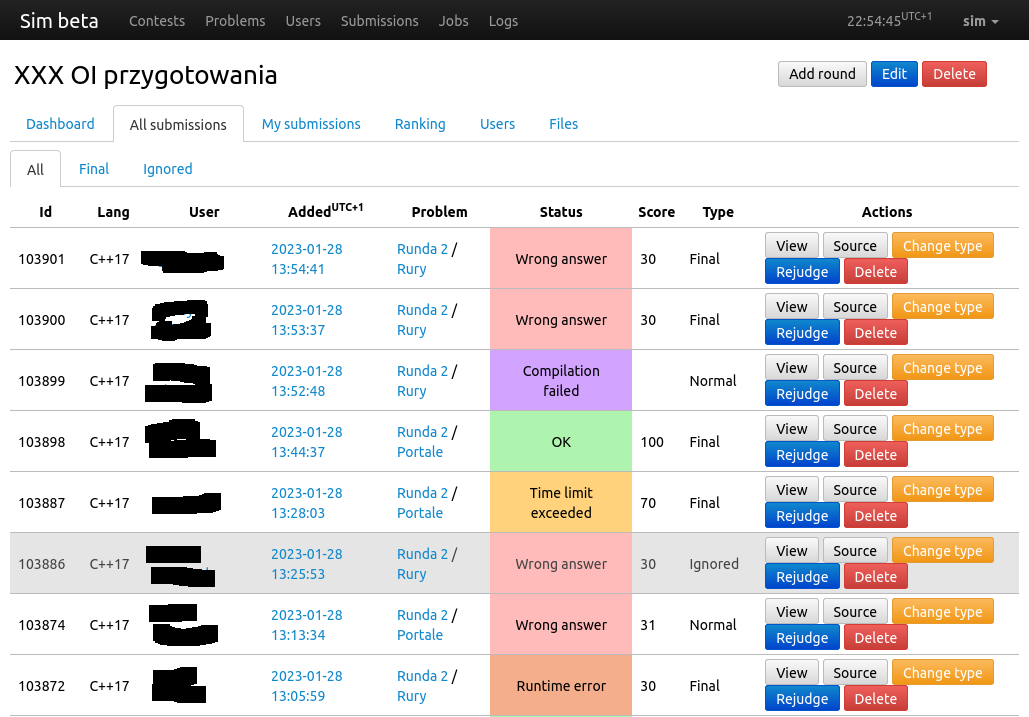
\includegraphics[height=8cm]{sim.png}
\end{frame}

\begin{frame}
    \frametitle{Before the new sandbox}

    \begin{block}{Old sandbox}
    \begin{itemize}
        \item Single-threaded, statically-linked executables
        \item C, C++, Pascal
        \item Overhead --- \texttt{ptrace}
    \end{itemize}
    \end{block}

    \begin{alertblock}{Problems}
    \begin{itemize}
        \item No support for other languages e.g. Python
        \item Compilation
    \end{itemize}
    \end{alertblock}

    \begin{exampleblock}{Solution}
    A new sandbox.
    \end{exampleblock}
\end{frame}

\begin{frame}
    \frametitle{The submission on the Sim platform}
    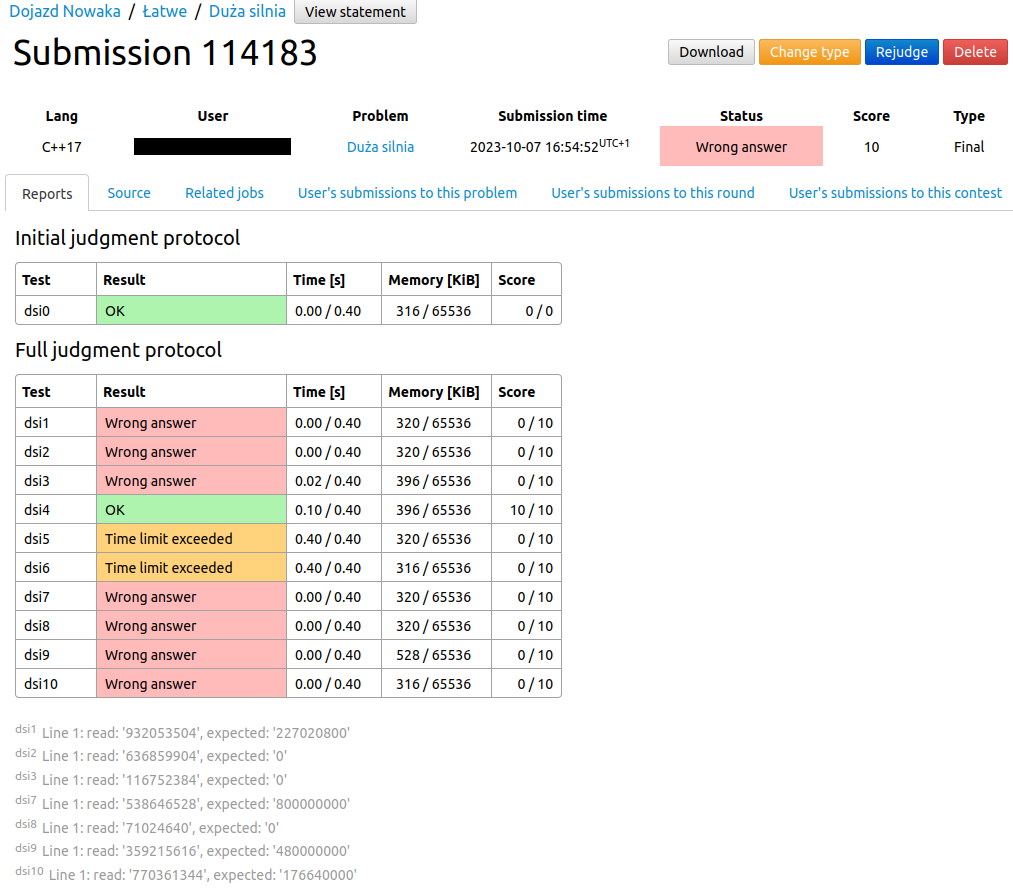
\includegraphics[height=8.5cm]{submission.png}
\end{frame}

\begin{frame}
    \frametitle{Requirements for new Sandbox}
    \begin{enumerate}
        \item Versatile
        \item Support for multi-process applications
        \item Low overhead
        \item Optimized for short-running programs
        \item Limiting resources
        \item Runtime statistics
        \item For unprivileged users
    \end{enumerate}
\end{frame}

\begin{frame}
    \frametitle{Existing solutions}
    \begin{itemize}
        \item Often require privileges e.g. OS modifications.
        \item Some use \texttt{ptrace}. Slow, TOCTOU problem.
        \item Few provide runtime statistics.
        \item \textcolor{red}{None is optimized for short-running programs.}
    \end{itemize}
\end{frame}

\begin{frame}[fragile]
    \frametitle{Design: client-server}

    Allows sharing resources between requests.

    \begin{figure}[h]
    \tikzset{>=latex} % set latex arrow tip
    \centering
    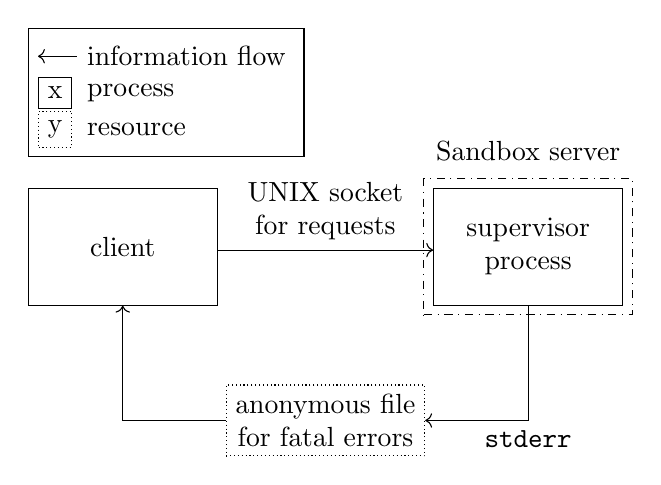
\begin{tikzpicture}[align=center]
        \node [draw, densely dotted] (errors) {anonymous file\\for fatal errors};
        \node [draw, above left=1cm and 0.1cm of errors, minimum height=1.4832815729996514cm, minimum width=2.4cm] (client) {client};
        \node [draw, above right=1cm and 0.1cm of errors, minimum height=1.4832815729996514cm, minimum width=2.4cm] (supervisor) {supervisor\\process};

        \draw[->] (client.-2) -- node[above] {UNIX socket \\ for requests} (supervisor.-178);
        \draw[<-] (client) |- node[below] {} (errors);
        \draw[->] (supervisor) |- node[below] {\texttt{stderr}} (errors);

        \begin{scope}[on background layer]
            \node [draw, dash dot, fit=(supervisor)] (server) {};
            \node [above=0.1cm of server] {Sandbox server};
        \end{scope}

        % Legend
        \matrix [draw, right] at ($(current bounding box.north west)+(0, 0.5)$) {
            \draw[<-] (0,0) -- (0.5,0); & \node[right] {information flow}; \\
            \draw node[right, draw] {x}; & \node[right] {process}; \\
            \draw node[right, draw, densely dotted] {y}; & \node[right] {resource}; \\
        };
    \end{tikzpicture}
    \end{figure}

    Benchmarks in a moment.

\end{frame}

\begin{frame}[fragile]
    \frametitle{Used Linux kernel mechanisms}
    Linux namespaces, cgroups, \texttt{prlimit}, seccomp BPF filters.

    \begin{figure}[h]
    \tikzset{>=latex} % set latex arrow tip
    \centering
    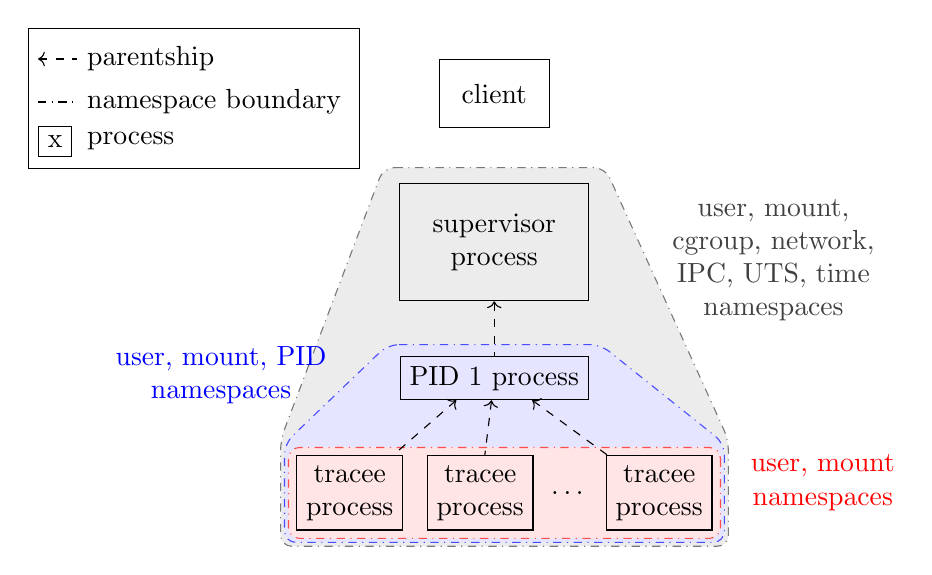
\begin{tikzpicture}[align=center, scale=0.5]
        \node [draw, minimum height=0.8652475842497965cm, minimum width=1.4cm] (client) {client};

        \node [draw, below=0.7cm of client, minimum height=1.4832815729996514cm, minimum width=2.4cm] (supervisor) {supervisor\\process};

        \node [draw, below=0.7cm of supervisor] (pid1) {PID~1 process};

        \node [draw, below left=0.7cm and -1.7cm of pid1] (tracee_mid) {tracee\\process};
        \node [draw, left=0.3cm of tracee_mid] (tracee_left) {tracee\\process};
        \node [right=0.1cm of tracee_mid] (tracee_dots) {\ldots};
        \node [draw, right=0.1cm of tracee_dots] (tracee_right) {tracee\\process};

        \draw[<-, dashed] (supervisor) -- (pid1);
        \draw[<-, dashed] (pid1) -- (tracee_mid);
        \draw[<-, dashed] (pid1.-150) -- (tracee_left);
        \draw[<-, dashed] (pid1.-30) -- (tracee_right);

        \begin{scope}[on background layer]
            \draw[dash dot, rounded corners, darkgray!70, fill=darkgray!10]
                ($(supervisor.north west)+(-0.4,0.4)$) --
                ($(supervisor.north east)+(0.4,0.4)$) -- node[above, xshift=12mm, pos=0.6, darkgray] {user, mount,\\cgroup, network,\\IPC, UTS, time\\namespaces}
                ($(tracee_right.north east)+(0.4,0.4)$) --
                ($(tracee_right.south east)+(0.4,-0.4)$) --
                ($(tracee_left.south west)+(-0.4,-0.4)$) --
                ($(tracee_left.north west)+(-0.4,0.4)$) --
                cycle;
        \end{scope}

        \begin{scope}[on background layer]
            \draw[dash dot, rounded corners, blue!70, fill=blue!10]
                ($(pid1.north west)+(-0.3,0.3)$) --
                ($(pid1.north east)+(0.3,0.3)$) --
                ($(tracee_right.north east)+(0.3,0.3)$) --
                ($(tracee_right.south east)+(0.3,-0.3)$) --
                ($(tracee_left.south west)+(-0.3,-0.3)$) --
                ($(tracee_left.north west)+(-0.3,0.3)$) -- node[above, xshift=-12mm, pos=0.3, blue] {user, mount, PID\\namespaces}
                cycle;
        \end{scope}

        \begin{scope}[on background layer]
            \draw[dash dot, rounded corners, red!70, fill=red!10]
                ($(tracee_right.north east)+(0.2,0.2)$) -- node[above, xshift=13mm, pos=0.8, red] {user, mount\\namespaces}
                ($(tracee_right.south east)+(0.2,-0.2)$) --
                ($(tracee_left.south west)+(-0.2,-0.2)$) --
                ($(tracee_left.north west)+(-0.2,0.2)$) --
                cycle;
        \end{scope}

        % Legend
        \matrix [draw, right] at ($(current bounding box.north west)+(-2, -1)$) {
            \draw[<-, dashed] (0,0) -- (0.5,0); & \node[right] {parentship}; \\
            \draw[-, dash dot] (0,0) -- (0.5,0); & \node[right] {namespace boundary}; \\
            \draw node[right, draw] {x}; & \node[right] {process}; \\
        };

    \end{tikzpicture}
    \end{figure}
\end{frame}

\begin{frame}
    \frametitle{Benchmark of some performance optimizations}
    \begin{scriptsize}
    \begin{table}
    \begin{tabular}{|l|r|r|r|r|}
    \hline
    \multicolumn{1}{|c|}{Benchmark} & \makecell{Mean\\request\\time} & \makecell{Std. dev.} & \makecell{Std. err.\\on the mean} & \multicolumn{1}{c|}{Slowdown} \\
    \hline
    Baseline                                              & 2.348ms & 0.768ms (32.71\%) & 0.024ms (1.03\%) & 0.00\% \\
    \hline
    \makecell{New network\\namespace \\ for each request}  & 2.970ms & 0.856ms (28.83\%) & 0.027ms (0.91\%) & 26.49\% \\
    \hline
    \makecell{New IPC\\namespace \\ for each request}      & 2.522ms & 0.782ms (31.02\%) & 0.025ms (0.98\%) & 7.41\% \\
    \hline
    \makecell{New UTS\\namespace \\ for each request}      & 2.478ms & 0.771ms (31.14\%) & 0.024ms (0.98\%) & 5.54\% \\
    \hline
    \multicolumn{1}{c}{}\\ % adds vertical space between table and caption
    \end{tabular}
    \caption{Statistics for each row were collected from 1000 runs. Each row contains real time it took to handle request to sandbox the \texttt{/bin/true} program.}
    \label{table:optimization_impact}
    \end{table}
    \end{scriptsize}
\end{frame}

\begin{frame}
    \frametitle{Comparison with nsjail}
    \begin{footnotesize}
    \begin{table}
    \begin{tabular}{|l|r|r|r|r|}
    \hline
    \makecell{Sandbox} & \makecell{Mean time} & \makecell{Std. dev.} & \makecell{Std. err.\\on the mean} & \makecell{Slowdown} \\
    \hline
    no sandbox   & 0.893ms & 0.409ms (45.80\%) & 0.013ms (1.45\%) & 1x \\
    sandbox      & 2.348ms & 0.768ms (32.71\%) & 0.024ms (1.03\%) & 2.39x \\
    nsjail       & 10.393ms & 1.327ms (12.77\%) & 0.042ms (0.40\%) & 10.57x \\
    \hline
    \multicolumn{1}{c}{}\\ % adds vertical space between tabular and caption
    \end{tabular}
    \caption{Statistics for each row were collected from 1000 runs. Each row contains real time it took to handle request to sandbox the \texttt{/bin/true} program. While the slowdown of the sandbox is huge (more than twofold), it still allows for hundreds of runs per second and that was the goal of this thesis, whereas nsjail is more than 4 times slower than our sandbox.}
    \end{table}
    \end{footnotesize}
\end{frame}

\begin{frame}
    \frametitle{Testing performance and overheads}
    Tested compilation of all solutions of 4 problems from finals of the XXII Polish Olimpiad in Informatics.
    \begin{itemize}
        \item Compilation.
        \item Running the model solution on the tests.
    \end{itemize}
    \begin{block}{Benchmark}
        Collect statistic from 10 runs.
    \end{block}
\end{frame}

\begin{frame}
    \frametitle{Compilation performance}
    Tested compilation of all solutions of 4 problems from finals of the XXII Polish Olimpiad in Informatics. 18 + 18 + 13 + 8 = 57 solutions.
    \begin{itemize}
        \item Only some compilations present statistically significant difference.
        \item \textcolor{green!70!black}{Half of the time it is statistically no slower that without the sandbox.}
        \item 0\% -- 24\% slowdown. Most of the time below 10\%.
        \item Almost always seccomp BPF filters cause the overhead (up to 15\% without it).
    \end{itemize}
\end{frame}

\begin{frame}
    \frametitle{Model solutions' performance}
    For each problem the single model solution was tested. Problems have: 55 + 57 + 69 + 65 = 246 tests.
    \begin{itemize}
        \item \textcolor{green!70!black}{Vast majority of tests shows no statistical difference.}
        \item Few test show slowdown --- up to 19\%.
        \item Medium tests even show speed-up --- up to 44\%.
        \item Low number of system calls. Most of the time, computations without IO.
    \end{itemize}
\end{frame}

\begin{frame}
    \frametitle{Future work}
    \begin{itemize}
        \item Setting CPU affinity
        \item Support for networking
        \item Rust frontend / client
        \item Further experimentation
    \end{itemize}
\end{frame}

\begin{frame}
    \begin{center}
        Thank you.
    \end{center}
\end{frame}

\begin{frame}[fragile]
    \frametitle{Bonus: IPC}

    \begin{figure}[h]
    \tikzset{>=latex} % set latex arrow tip
    \centering
    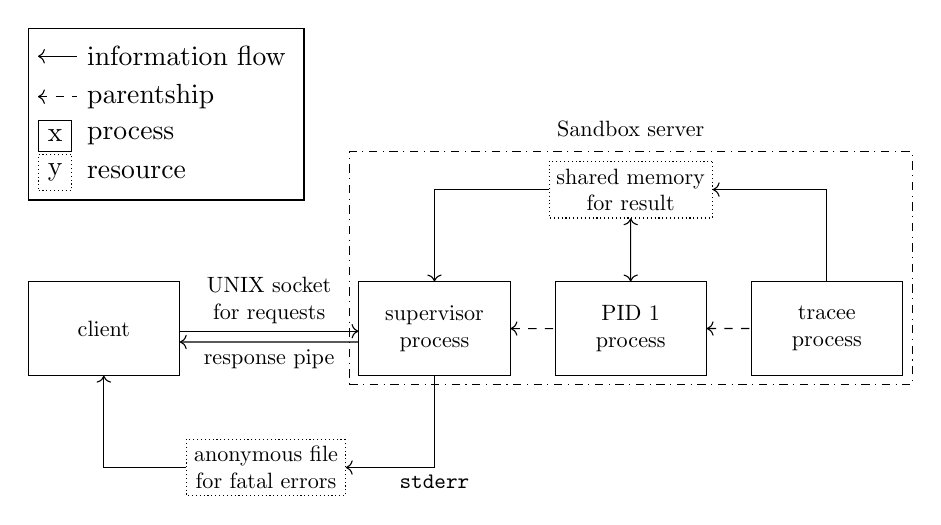
\begin{tikzpicture}[align=center,scale=0.8, every node/.style={transform shape}]
        \node [draw, densely dotted] (errors) {anonymous file\\for fatal errors};
        \node [draw, above left=1cm and 0.1cm of errors, minimum height=1.4832815729996514cm, minimum width=2.4cm] (client) {client};
        \node [draw, above right=1cm and 0.2cm of errors, minimum height=1.4832815729996514cm, minimum width=2.4cm] (supervisor) {supervisor\\process};

        \node [draw, right=0cm and 0.7cm of supervisor, minimum height=1.4832815729996514cm, minimum width=2.4cm] (pid1) {PID~1\\process};

        \node [draw, right=0cm and 0.7cm of pid1, minimum height=1.4832815729996514cm, minimum width=2.4cm] (tracee) {tracee\\process};

        \node [draw, above=1cm of pid1, densely dotted] (shmem) {shared memory\\for result};

        \draw[->] (client.-2) -- node[above] {UNIX socket \\ for requests} (supervisor.-178);
        \draw[<-] (client.-10) -- node[below] {response pipe} (supervisor.-170);
        \draw[<-] (client) |- node[below] {} (errors);
        \draw[->] (supervisor) |- node[below] {\texttt{stderr}} (errors);
        \draw[<-] (supervisor.north) |- (shmem);
        \draw[<->] (shmem.south) -- (pid1.north);
        \draw[<-] (shmem.east) -| (tracee.north);
        \draw[<-, dashed] (supervisor) -- (pid1);
        \draw[<-, dashed] (pid1) -- (tracee);

        \begin{scope}[on background layer]
            \node [draw, dash dot, fit=(supervisor) (pid1) (shmem) (tracee)] (server) {};
            \node [above=0.1cm of server] {Sandbox server};
        \end{scope}

        % Legend
        \matrix [draw, right] at (current bounding box.north west) {
            \draw[<-] (0,0) -- (0.5,0); & \node[right] {information flow}; \\
            \draw[<-, dashed] (0,0) -- (0.5,0); & \node[right] {parentship}; \\
            \draw node[right, draw] {x}; & \node[right] {process}; \\
            \draw node[right, draw, densely dotted] {y}; & \node[right] {resource}; \\
        };

    \end{tikzpicture}
    \end{figure}
\end{frame}

\begin{frame}
    \frametitle{Bonus: Implementation}

    \begin{enumerate}
        \item Time limits
        \item Runtime statistics
        \item Error handling (stderr)
        \item Request sending and receiving (serialization)
        \item File descriptors
        \item Cancelling or killing request
        \item Sandbox server upon client death
        \item PID 1 process upon supervisor death
        \item Signals (tracee, SIGPIPE, UBSan)
        \item Running as superuser
        \item Performance optimizations
    \end{enumerate}
\end{frame}

\end{document}
